\begin{figure}[!ht]
  \centering
  \begingroup
  \pgfplotsset{
    io timing/.style={
      width=0.48\linewidth, height=0.28\linewidth,
      xmin=-0.18, ymin=0, enlarge x limits=false,
      ylabel={Time (s)}, xlabel={MPI ranks},
      grid=major, grid style={gray!20},
      label style={font=\small}, title style={font=\small},
      tick label style={font=\footnotesize},
      legend style={font=\scriptsize, draw=none, inner sep=1pt},
      legend pos=north west, legend cell align=left,
      every axis plot/.append style={thick,mark size=1.5pt}
    },
    io mesh/.style={blue!75!black, mark=*},
    io mesh read/.style={blue!75!black, dashed, mark=o},
    io field/.style={red!65!black, mark=square*},
    io field read/.style={red!65!black, dashed, mark=square},
    io fixed/.style={xmax=3.18,xtick={0,1,2,3},xticklabels={256,512,1024,2048}},
    io weak a/.style={xmax=4.18,xtick={0,1,2,3,4},xticklabels={256,512,1024,2048,4096}},
    io weak b/.style={xmax=4.18,xtick={0,1,2,3,4},xticklabels={512,1024,2048,4096,8192}}
  }
  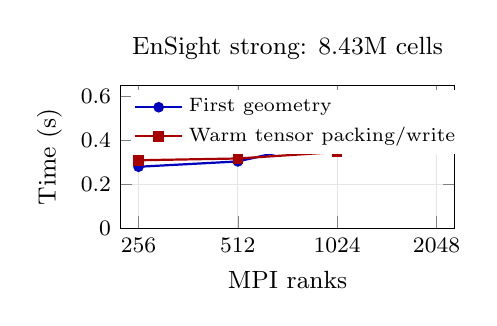
\begin{tikzpicture}
    \begin{axis}[io timing,io fixed,title={EnSight strong: 8.43M cells},ymax=.65]
      \addplot[io mesh] coordinates {(0,.279757) (1,.304032) (2,.406130) (3,.512470)};
      \addlegendentry{First geometry}
      \addplot[io field] coordinates {(0,.309313) (1,.317408) (2,.346909) (3,.417139)};
      \addlegendentry{Warm tensor packing/write}
    \end{axis}
  \end{tikzpicture}%
  \hfill
  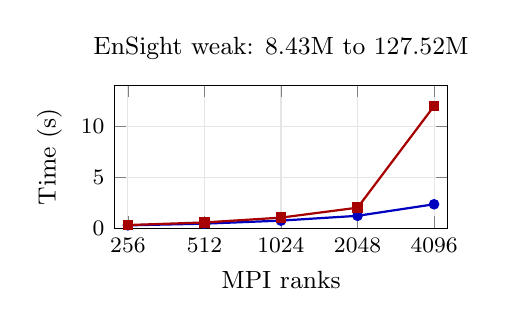
\begin{tikzpicture}
    \begin{axis}[io timing,io weak a,title={EnSight weak: 8.43M to 127.52M},ymax=14]
      \addplot[io mesh] coordinates {(0,.279757) (1,.446706) (2,.744355) (3,1.216125) (4,2.347226)};
      \addplot[io field] coordinates {(0,.309313) (1,.564948) (2,1.038139) (3,2.012444) (4,11.977646)};
    \end{axis}
  \end{tikzpicture}

  \medskip
  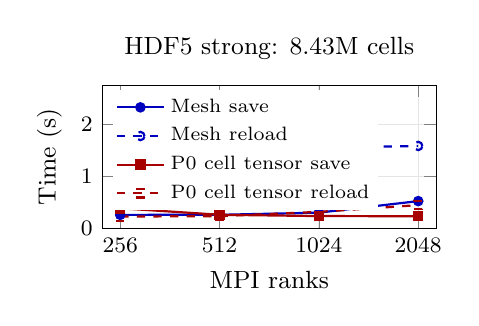
\begin{tikzpicture}
    \begin{axis}[io timing,io fixed,title={HDF5 strong: 8.43M cells},ymax=2.75]
      \addplot[io mesh] coordinates {(0,.257) (1,.258) (2,.300) (3,.522)};
      \addlegendentry{Mesh save}
      \addplot[io mesh read] coordinates {(0,1.522) (1,1.239) (2,1.548) (3,1.584)};
      \addlegendentry{Mesh reload}
      \addplot[io field] coordinates {(0,.384) (1,.259) (2,.234) (3,.231)};
      \addlegendentry{P0 cell tensor save}
      \addplot[io field read] coordinates {(0,.225) (1,.232) (2,.315) (3,.445)};
      \addlegendentry{P0 cell tensor reload}
    \end{axis}
  \end{tikzpicture}%
  \hfill
  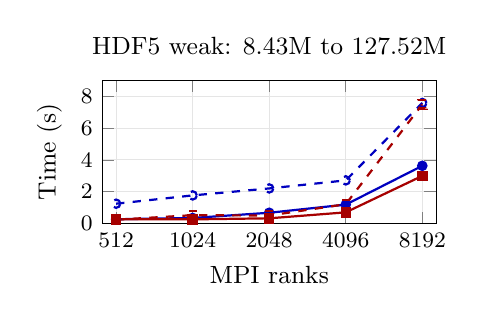
\begin{tikzpicture}
    \begin{axis}[io timing,io weak b,title={HDF5 weak: 8.43M to 127.52M},ymax=9]
      \addplot[io mesh] coordinates {(0,.258) (1,.340) (2,.668) (3,1.181) (4,3.628)};
      \addplot[io mesh read] coordinates {(0,1.239) (1,1.762) (2,2.202) (3,2.709) (4,7.589)};
      \addplot[io field] coordinates {(0,.259) (1,.252) (2,.318) (3,.694) (4,2.993)};
      \addplot[io field read] coordinates {(0,.232) (1,.515) (2,.494) (3,1.207) (4,7.498)};
    \end{axis}
  \end{tikzpicture}
  \endgroup
  \caption{Discoverer/Lustre scaling with nodal P1 and DG P0, one
    verified run per point. Top: rank-zero EnSight, first geometry
    write and second-frame cell-tensor packing and write (maximum rank
    time). Bottom: native HDF5 mesh and cell-tensor save and immediate
    exact reload. The weak series use about 31,000--33,000 cells per
    rank for EnSight and 15,500--16,500 for HDF5. Legends apply
    across each row.}
  \label{fig:app-feelpp-io:scaling-by-operation}
\end{figure}
